\documentclass[12pt]{beamer}

\usepackage{pdfpages}
\usepackage{xeCJK}
\setCJKmainfont{STHeiti}
\setCJKsansfont{STKaiti}
\newcommand{\kaiti}{\fontfamily{STKaiti}\selectfont}
\newcommand{\heiti}{\fontfamily{STHeiti}\selectfont}

\usepackage{inputenc}
\usepackage{varwidth}
\usepackage{xcolor}
\definecolor{colora}{RGB}{214,76,71}
\definecolor{colorg}{RGB}{84,175,216}
\definecolor{colort}{RGB}{98,174,17}
\definecolor{colorc}{RGB}{253,205,103}
\definecolor{colorn}{RGB}{ 45,45,45}
\definecolor{colord}{RGB}{ 44,46,255}
\definecolor{colorb}{RGB}{ 14,41,89}
\definecolor{colori}{RGB}{255,44,45}
\definecolor{beaublue}{rgb}{0.74, 0.83, 0.9}
\definecolor{backg}{RGB}{30, 60, 150}

\usepackage{adjustbox}
\usepackage{tikz}
\usetikzlibrary{arrows,shapes,backgrounds,shadows,decorations.pathreplacing,decorations.pathmorphing}
\tikzstyle{every picture}+=[remember picture]
\tikzstyle{na} = [baseline=-.5ex]
\tikzstyle{block} = [ultra thick, align=left, rounded corners, drop shadow, draw=black, fill=colorn,text=white]
\tikzstyle{refbg} = [rounded corners, text width=\textwidth, fill=beaublue]

\tikzstyle{elec} = [line width=2pt,draw=black!80]
\tikzstyle{vib} = [thick,draw=black!30]
\tikzstyle{relax} = [draw=orange,ultra thick,decorate,decoration=snake]

\tikzstyle{blockA} = [fill=colora, draw=black, ultra thick, rounded corners, drop shadow,text=white]
\tikzstyle{blockC} = [fill=colorc, draw=black, ultra thick, rounded corners, drop shadow,text=white]
\tikzstyle{blockG} = [fill=colorg, draw=black, ultra thick, rounded corners, drop shadow,text=white]
\tikzstyle{blockT} = [fill=colort, draw=black, ultra thick, rounded corners, drop shadow,text=white]
\tikzstyle{blockN} = [fill=colorn, draw=black, ultra thick, rounded corners, drop shadow,text=white]
\tikzstyle{blockd} = [fill=colord, draw=black, ultra thick, rounded corners, drop shadow,text=white]
\tikzstyle{blockb} = [fill=colorb, draw=black, ultra thick, rounded corners, drop shadow,text=white]
\tikzstyle{blocki} = [fill=colori, draw=black, ultra thick, rounded corners, drop shadow,text=white]

\tikzstyle{circleA} = [circle, inner color = colora!20, outer color=colora, draw=black, ultra thick, rounded corners, drop shadow]
\tikzstyle{circleC} = [circle, inner color = colorc!20, outer color=colorc, draw=black, ultra thick, rounded corners, drop shadow]
\tikzstyle{circleG} = [circle, inner color = colorg!20, outer color=colorg, draw=black, ultra thick, rounded corners, drop shadow]
\tikzstyle{circleT} = [circle, inner color = colort!20, outer color=colort, draw=black, ultra thick, rounded corners, drop shadow]
\tikzstyle{circleN} = [circle, inner color = colorn!20, outer color=colorn, draw=black, ultra thick, rounded corners, drop shadow]
\tikzstyle{circled} = [circle, inner color = colord!20, outer color=colord, draw=black, ultra thick, rounded corners, drop shadow]
\tikzstyle{circleb} = [circle, inner color = colorb!20, outer color=colorb, draw=black, ultra thick, rounded corners, drop shadow]
\tikzstyle{circlei} = [circle, inner color = colori!20, outer color=colori, draw=black, ultra thick, rounded corners, drop shadow]

\pgfmathdeclarerandomlist{randomColors}{
  {colora}
  {colorc}
  {colorg}
  {colort}
}

\pgfmathdeclarerandomlist{randomBlocks}{
  {blockA}
  {blockC}
  {blockG}
  {blockT}
}

\usepackage{tcolorbox}
\usepackage{listings}

%\setbeamertemplate{sections in toc}[circle]
\usetheme{Frankfurt}
\usecolortheme[named=backg]{structure}
\setbeamertemplate{sections/subsections in toc}[circle]
\setbeamertemplate{itemize items}[triangle]

\setbeamertemplate{footline}{

\includegraphics[height=1.5em]{figures/copyright.png}
    \hfill
    \insertframenumber
    /
    \inserttotalframenumber
    \hspace{0.1cm}
}



\title{\huge{全基因组与目标区域DNA重测序数据分析}}
\author{\large{石\ 泉}\\shiquan@genomics.cn\\https://github.com/shiquan}
\institute{\large{华大基因研究院}}
\date{}
\begin{document}
\frame{\titlepage}
\begin{frame}{前言}
  \kaiti{本文档为华大学院组织培训《全基因组与目标区域DNA重测序数据
      分析》课程授课课件。进入课程讨论前,假设学员已经对一下内容予以了解。}
 \begin{columns}
 \begin{column}{0.35\textwidth}
 \begin{itemize}
 \item 生物基础 \tikz \coordinate (l-i1);
 \item 测序原理 \tikz \coordinate (l-i2);
 \item Linux\\操作基础 \tikz \coordinate (l-i3);
 \end{itemize}
 \end{column}
 \begin{column}{0.65\textwidth}
 \begin{itemize}
\item \tikz \coordinate (r-i1); 中心法则(center dogma)
\item \tikz \coordinate (r-i2); DNA packaging 
\item \tikz \coordinate (r-i3); cDNA, noncoding RNA 
\item \tikz \coordinate (r-i4); 读长(reads),接头(adaptor) 
\item \tikz \coordinate (r-i5); barcoding 
\item \tikz \coordinate (r-i6); 解压压缩包 
\item \tikz \coordinate (r-i7); GNU Make,GCC 
 \end{itemize}
 \end{column}
 \end{columns}
 \begin{tikzpicture}[overlay]
 \path[->,colora,ultra thick] (l-i1) edge [in=180, out=0] (r-i1);
 \path[->,colora,ultra thick] (l-i1) edge [in=180, out=0] (r-i2);
 \path[->,colora,ultra thick] (l-i1) edge [in=180, out=0] (r-i3);
 \path[->,colorc,ultra thick] (l-i2) edge [in=180, out=0] (r-i4);
 \path[->,colorc,ultra thick] (l-i2) edge [in=180, out=0] (r-i5);
 \path[->,colorn,ultra thick] (l-i3) edge [in=180, out=0] (r-i6);
 \path[->,colorn,ultra thick] (l-i3) edge [in=180, out=0] (r-i7);
 \end{tikzpicture}
 \end{frame}
\defverbatim[colored]\unp{
\begin{lstlisting}[language=bash,basicstyle=\ttfamily,keywordstyle=\color{red}]
  $ cd sources 
  $ ls
  bcftools-1.3.tar.bz2  bwa-0.7.13.tar.bz2    samtools-1.3.tar.bz2
  $ tar jxvf bcftools-1.3.tar.bz2
  $ cd bcftools-1.3
  $ make
  $ cd .. 
  $ tar jxvf bwa-0.7.13.tar.bz2
  $ tar jxvf samtools-1.3.tar.bz2 
\end{lstlisting}
}
\begin{frame}\frametitle{预备工作:解压源代码及编译}
  \unp

  如对以上命令不了解,请参考《鸟哥的Linux私房菜》。
  
\end{frame}
\begin{frame}\frametitle{目录}
 \tableofcontents
 \end{frame}

\section{什么是DNA重测序?}
\begin{frame}\frametitle{什么是DNA''重''测序?}
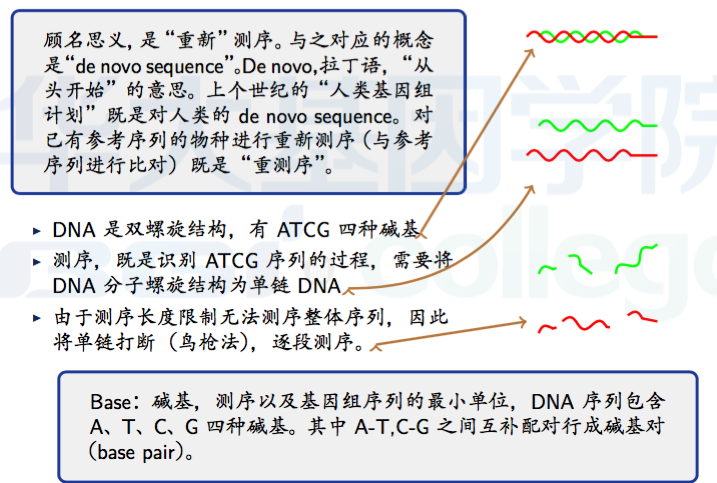
\includegraphics[width=\textwidth]{figures/old_slides/reseq.png}
\end{frame}


\section{为什么进行重测序?}
\begin{frame}\frametitle{为什么进行DNA重测序?}
  \begin{columns}
    \begin{column}{0.5\textwidth}
      \begin{itemize}
      \item 环境因素和遗传因素作用导致疾病。
      \item 器质性病变无法逆转(大叶性肺炎除外)。
      \item 蛋白测序、RNA测序难度远高于DNA测序。
      \item DNA检测的优势和适用。
      \item 早发现,早治疗。未病先防。        
      \end{itemize}
      \end{column}
    \begin{column}{0.5\textwidth}
      \includegraphics[width=\textwidth]{figures/bio_layer.pdf}
      \end{column}
    \end{columns}
  \end{frame}

\begin{frame}\frametitle{研究遗传性状(表型)的一般步骤\ref{ref1}}
  \begin{enumerate}
  \item Recognition of the disease state or syndrome, including assessment of its hereditary character;
  \item Discovery and mapping of the related polymorphism(s) or mutation(s);
  \item Elucidation of the biochemical/biophysical mechanism leading to the disease phenotype.
  \end{enumerate}
\begin{center}
  \begin{tikzpicture}
    \node[blockA] (n1) at (0,0) {表型};
    \node[blockT] (n2) at (5,0) {变异信息};
    \node[blockG] (n3) at (3,2) {致病机制};

    \node[blockC] (n4) at (2.5,0){};
    \draw[-, ultra thick, draw=backg] (n1) -- (n4);
    \draw[-, ultra thick, draw=backg] (n2) -- (n4);
    \draw[->, ultra thick, draw=backg, in = 180, out=90] (n4) -- (n3);
  \end{tikzpicture}
\end{center}
  \tikz \node[refbg]{
    \begin{thebibliography}{}
      {\small{\bibitem[Michael R. Barnes]{ref1} Michael R. Barnes. \emph{Bioinformatics for Geneticists 2nd}, 2006, P4-5.}}
    \end{thebibliography}
  };

  
  \end{frame}

\begin{frame}\frametitle{研究对象}
  \begin{itemize}
  \item 物种? (人、细菌)
  \item 组织? (正常组织细胞、血液、癌细胞)
  \item 健康状况? (正常人筛查、患者辅助诊断)
  \item 样品特征? (干血片)
  \end{itemize}
  \end{frame}

\begin{frame}\frametitle{遗传变异基础}
  根据变异范围划分:
  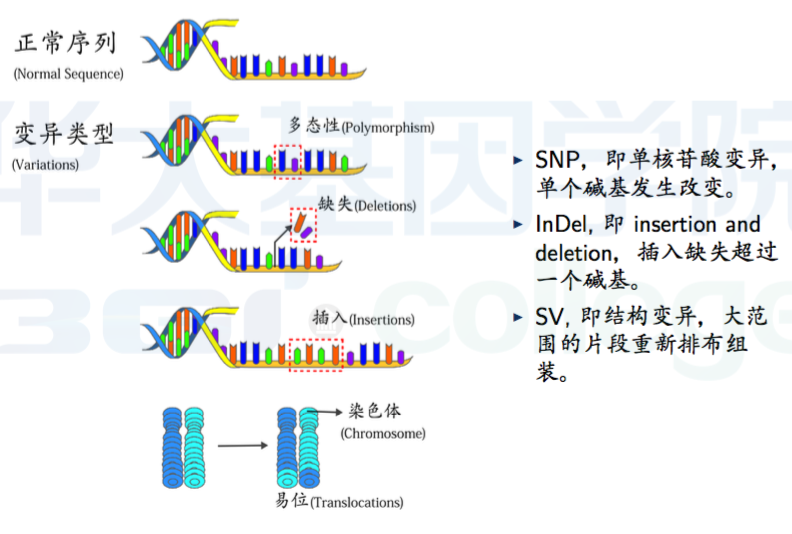
\includegraphics[width=\textwidth]{figures/old_slides/varbasic.png}
\end{frame}

\begin{frame}\frametitle{Germline and somatic (driver) mutations}
    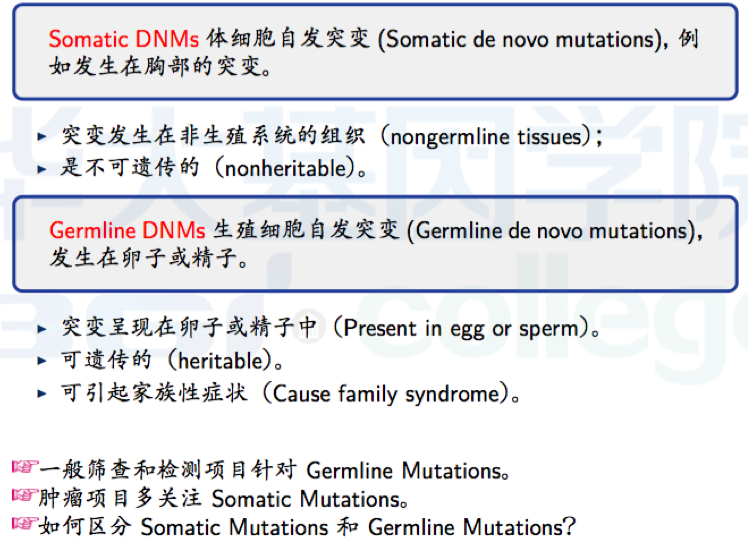
\includegraphics[width=\textwidth]{figures/old_slides/vartype.png}
  \end{frame}


\begin{frame}%\frametitle{SNV}
  \begin{center}
    {  \large  SNVs = SNPs + Point mutations}
  \end{center}
  {\small
\begin{tcolorbox}[colback=backg!5,colframe=backg,title=SNV]
  SNV 单核苷酸变异 (Single Nucleotide Variation), a single base insertion or deletion, a transition or transversion. Includes the set of SNPs.
\end{tcolorbox}
\begin{tcolorbox}[colback=backg!5,colframe=backg,title=SNP]
  SNP单核苷酸多态性(Single Nucleotide Polymorphism),指的是DNA序列上发生的单个核苷酸碱基之间的变异。在人群中这种编译的发生频率至少大于1\%,否则被认为是点突变。“在人类遗传基因的各种差异,有90\%都可归因于SNP所引起的基因变异。在人基因组中,每隔100至300个碱基就会存在一处SNP。每3个SNP中有两个会是胞嘧啶(C)和胸腺嘧啶(T)的相互转变。”
  \end{tcolorbox}
  }

\end{frame}

\begin{frame}
  \begin{tcolorbox}[colback=backg!5,colframe=backg,title=Point mutations]
   Point Mutation 点突变,是突变的一种类型,会使单一个碱基核 苷酸替换成另一种核苷酸,一般也包括只有作用于单一剪辑对 的插入或者缺失。在人群的发生率小于 1\%,与之相对的定义是 SNP(见上一页)。
  \end{tcolorbox}
  突变可依发生位置对基因功能的影响而作以下分类:
  \begin{itemize}
  \item 无义突变 (nonsense mutation),使原本可编码蛋白的密码子变成终止密码。
  \item 错义突变 (missense mutation),使密码子对应的编码氨基酸发生改变。
  \item 沉默突变 (silent mutation),密码子改变,但编码氨基酸不变。
  \end{itemize}
\end{frame}

\begin{frame}\frametitle{Insert and Deletion}
  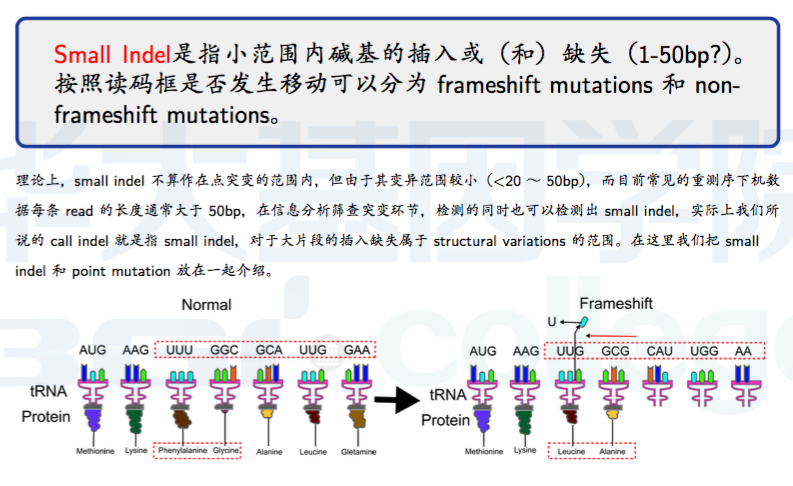
\includegraphics[width=\textwidth]{figures/old_slides/indel.png}
\end{frame}

\begin{frame}\frametitle{Splice sites}
  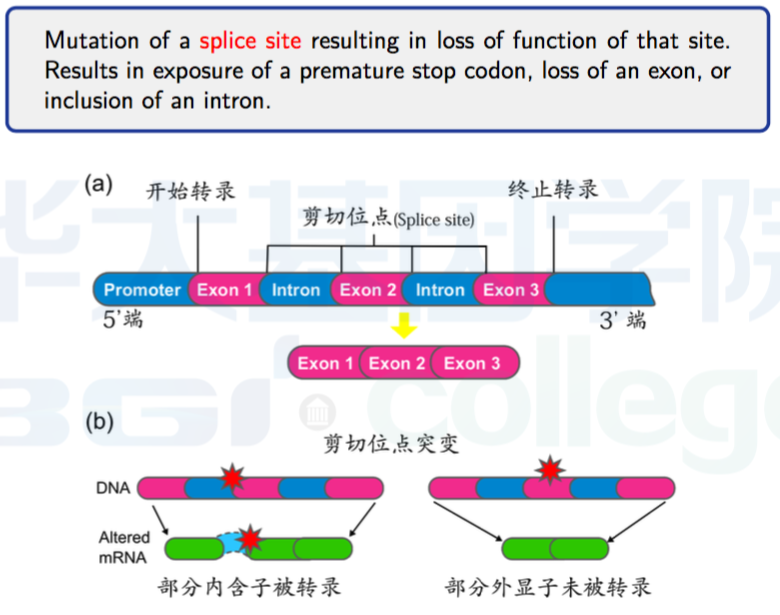
\includegraphics[width=\textwidth]{figures/old_slides/splice.png}
\end{frame}

\begin{frame}\frametitle{Structure variantion (SV)}
  \begin{itemize}
  \item Unbalanced SV
    \begin{itemize}
    \item Copy number variantion
    \item Novo insertion
    \end{itemize}
  \item Balanced SV
    \begin{itemize}
    \item Inversion
    \item Translocation
    \end{itemize}
  \item Aneuploidies
  \end{itemize}
\end{frame}

\begin{frame}\frametitle{CNV}
  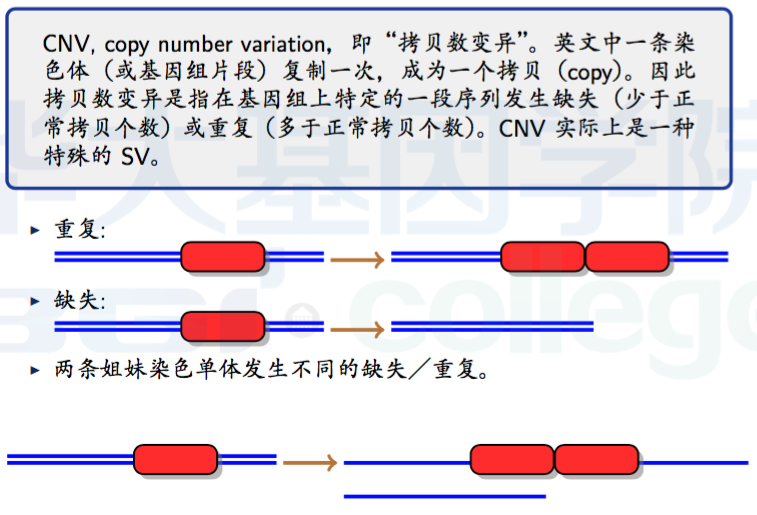
\includegraphics[width=\textwidth]{figures/old_slides/cnv.png}
\end{frame}

\section{如何进行重测序?}
\begin{frame}\frametitle{如何进行重测序?}
  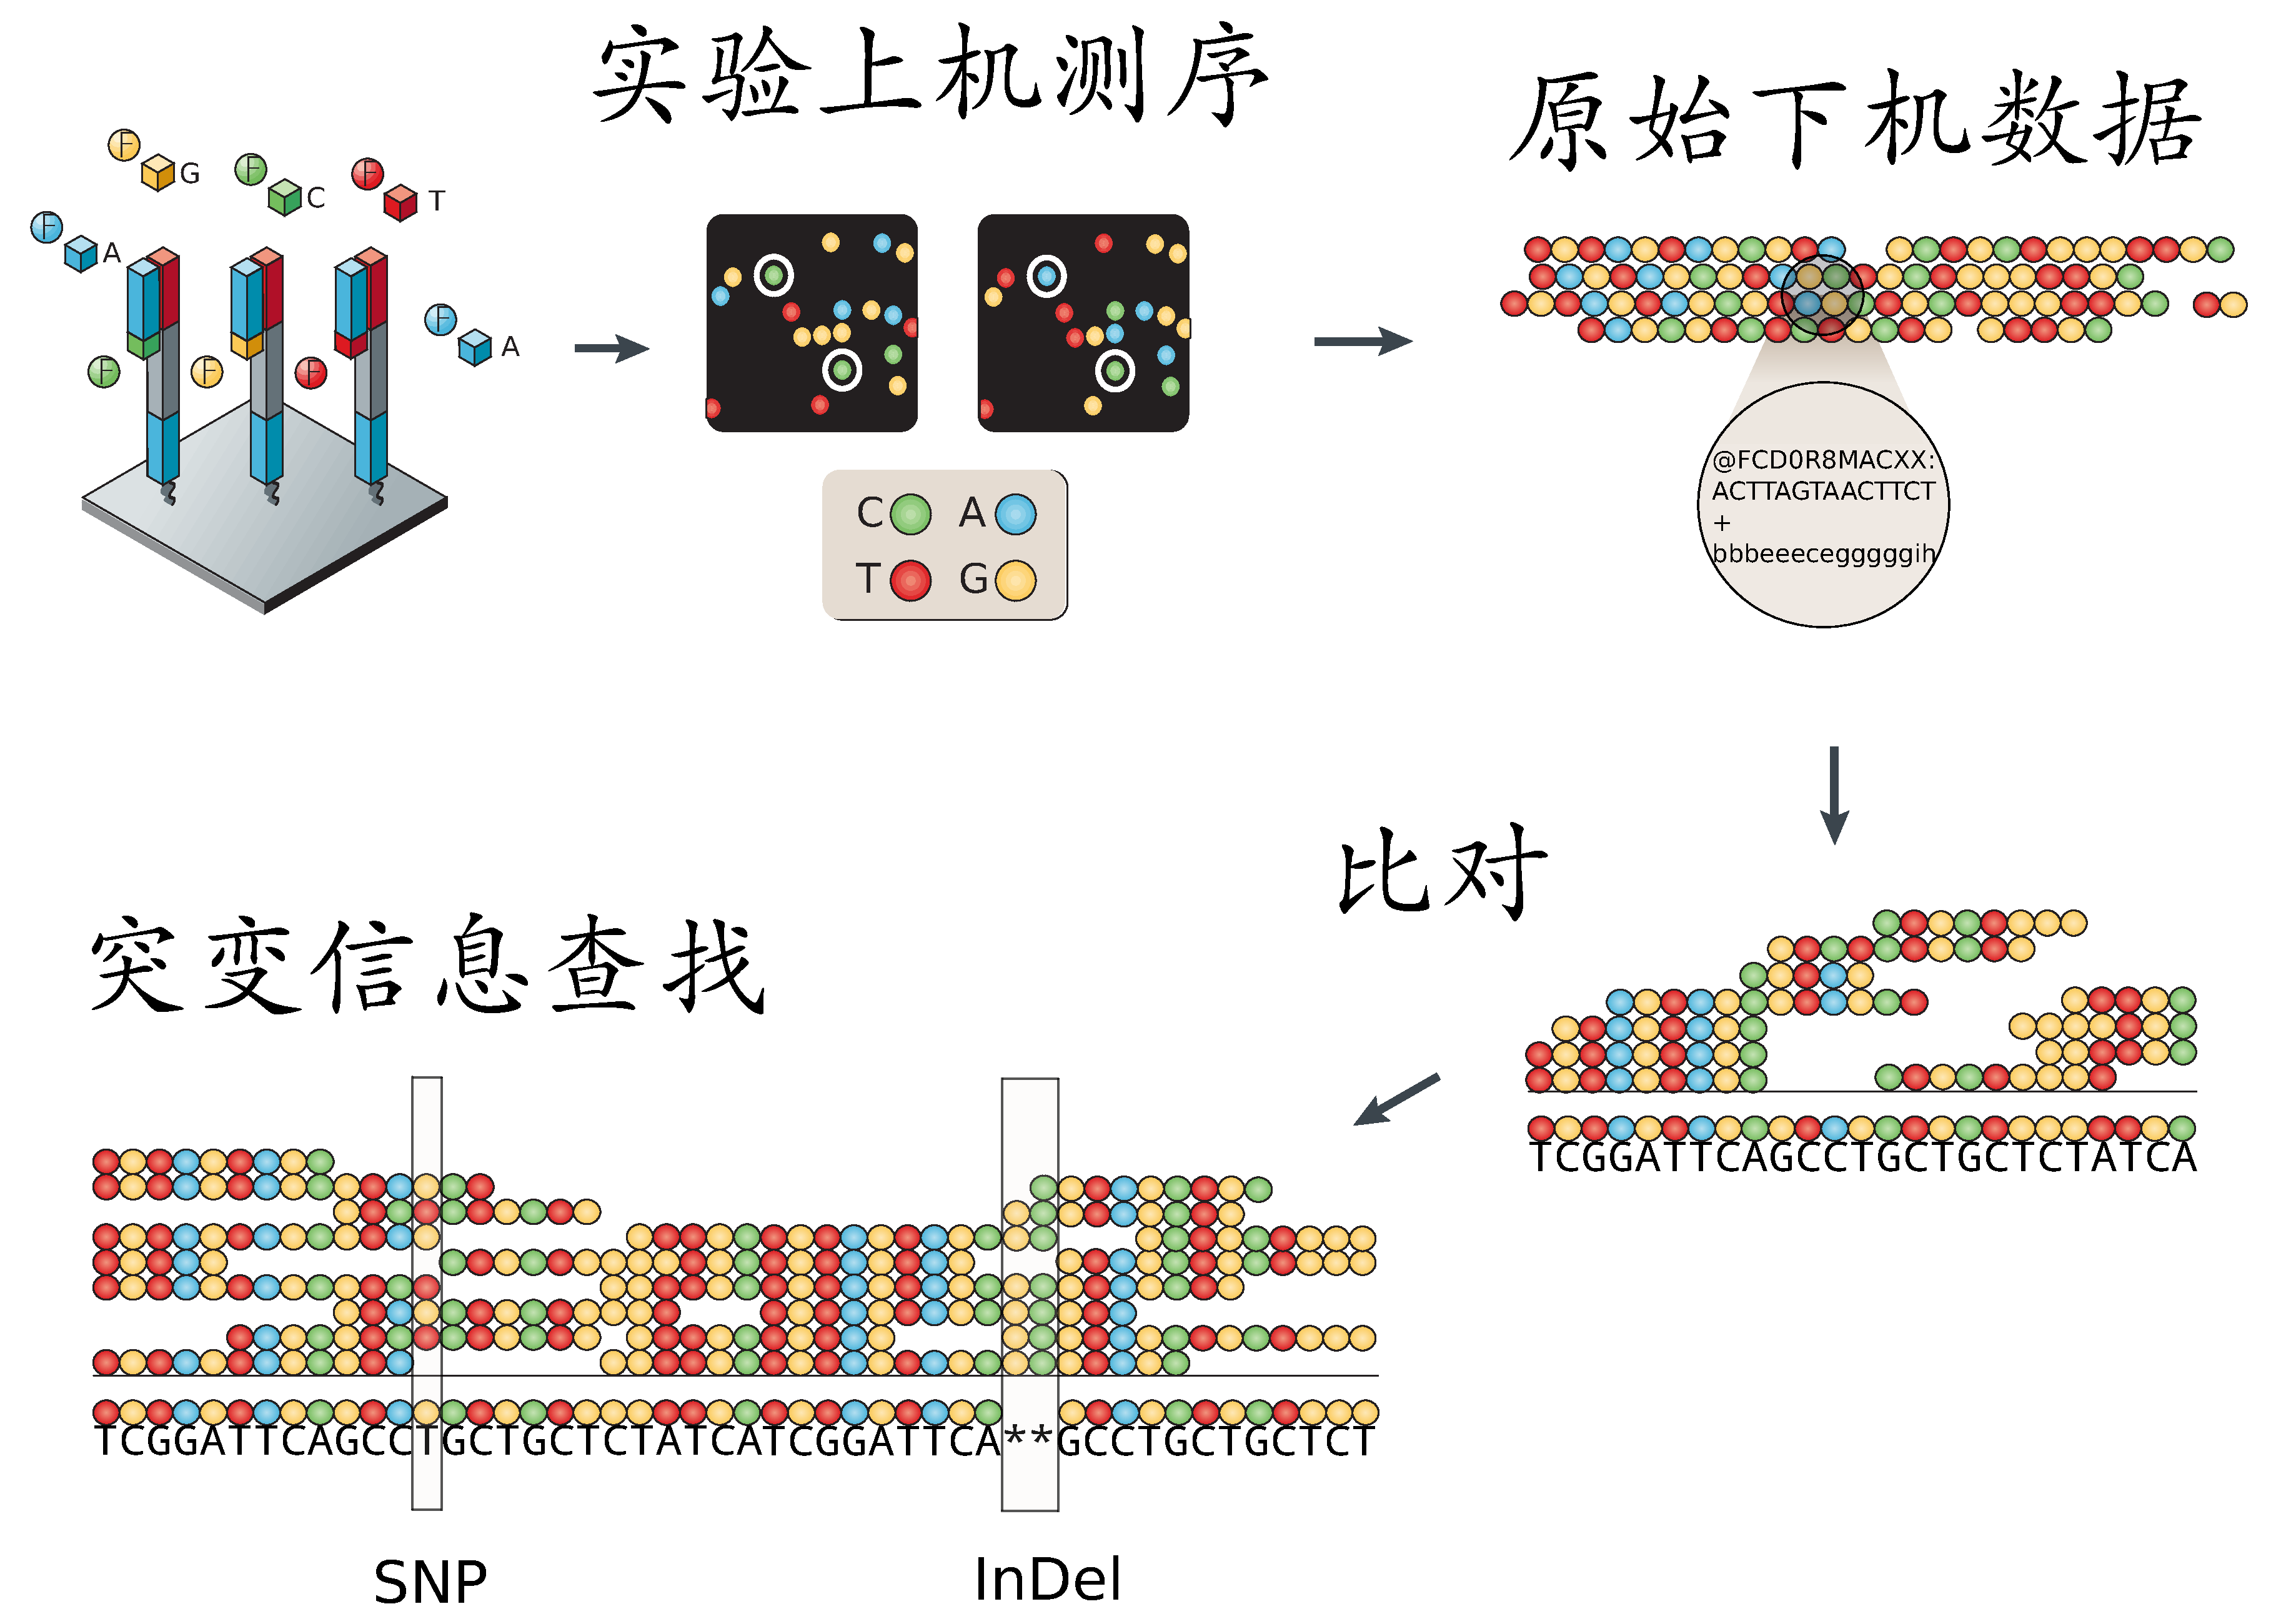
\includegraphics[width=\textwidth]{figures/reseq-pip.png}
\end{frame}

\begin{frame}
  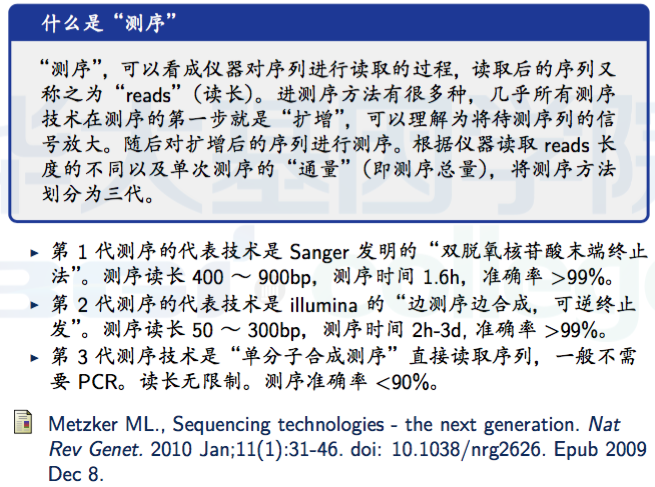
\includegraphics[width=\textwidth]{figures/old_slides/seq.png}
\end{frame}

\begin{frame}\frametitle{几张常见的重测序建库方法}
  \begin{enumerate}
  \item 全基因组测序;
    \begin{itemize}
    \item 不需要富集,建库步骤相对简单
    \item 测序数据量大,一般测序仪很难满足通量需求(3.2G,30x)
    \item 变异信息全面但信息分析速度较慢
    \item 适合检测大范围结构的缺失和重复以及染色体变异
    \end{itemize}
    
  \item 基于目标序列的芯片捕获测序;
    \begin{itemize}
    \item 设计灵活,可根据不同目的基因调整捕获区域
    \item 成本远低于全基因组测序(30M vs 3.2G)
    \item 受制于探针设计技术,不同基因组序列复杂度区域捕获效果差异大
    \end{itemize}
  \item 目标区域 PCR 扩增测序。
    \begin{itemize}
    \item 对引物扩增效率要求高
    \item PCR 富集效果一般好于芯片捕获
    \item 受制于引物条数限制,测序目标区域往往是单个或特定个数区域
    \end{itemize}
  \end{enumerate}
\end{frame}

\begin{frame}\frametitle{常见测序方法}
  \begin{tcolorbox}[colback=backg!5,colframe=backg,title=测序方法]
    除了测序原理有所不同,不同的平台测序方式亦有很大差异。根据测序结果文件,最常见的测序方案可以分为“SE”和“PE”两种。除此之外还有其他类型的测序形式(如CG的dnb测序)。
  \end{tcolorbox}
  \begin{itemize}
    \item Single end(SE),即单端测序,这是常见的测序方式, 从一条序列的一端开始读取,直到测序终止 。
    \item Paired end(PE),即双端测序。 从一条序列的一端开始读取 ,同时或者之后 从该序列的另一端再读取一次 。 即对一条序列分别从两端,共进行了两次的读取。
\end{itemize}
\end{frame}

\begin{frame}
  Single end测序会输出一个测序文件。
  \begin{adjustbox}{width=\textwidth}
    \begin{tikzpicture}
      \begin{scope}
  \foreach \x in {0, 0.5, ..., 5 }
  \shade[circle, outer color = colorn, inner color = colorn!20, thick, draw=black] (\x,2-\x*2*0.2) circle(0.25);
 
  \foreach \x in {5.5, 6, ..., 12.5 }
   \pgfmathrandomitem{\nucl}{randomColors} 
   \shade[circle, outer color = \nucl, inner color = \nucl!20, thick, draw=black] (\x, 0) circle(0.25);
   \foreach \x in {13, 13.5, ..., 25 }
   \shade[circle, outer color = colorn, inner color = colorn!20, thick, draw=black] (\x, 0) circle(0.25);

   \draw[decorate,decoration={brace,mirror,raise=10,amplitude=20}, ultra thick, draw=black] (0, 2) -- (5, 0) node [midway,below,sloped,yshift=-30,xshift=-10]{\bfseries{adaptor, barcode sequences}};
   \draw[->, blue,ultra thick] (0,2.5) -- (5,0.5) -- (12.5,0.5);
   \node[blockN] at (5,2) {\huge{Read1}};
   \draw[white] (-2,-2) rectangle (34,4);
      \end{scope}
    \end{tikzpicture}
  \end{adjustbox}



  Pair end测序会输出一对(两个)测序文件。
  \begin{adjustbox}{width=\textwidth}
    \begin{tikzpicture}
\begin{scope}
  \foreach \x in {0, 0.5, ..., 5 }
  \shade[circle, outer color = colorn, inner color = colorn!20, thick, draw=black] (\x,2-\x*2*0.2) circle(0.25);
  \foreach \x in {5.5, 6, ..., 12.5 }
   \pgfmathrandomitem{\nucl}{randomColors} 
   \shade[circle, outer color = \nucl, inner color = \nucl!20, thick, draw=black] (\x, 0) circle(0.25);
   \foreach \x in {13, 13.5, ..., 20 }
  \shade[circle, outer color = colorn, inner color = colorn!20, thick, draw=black] (\x, 0) circle(0.25);
   \foreach \x in {20.5, 21, ..., 27.5 }
   \pgfmathrandomitem{\nucl}{randomColors}
   \shade[circle, outer color = \nucl, inner color = \nucl!20, thick, draw=black] (\x, 0) circle(0.25);
   \foreach \x in {0, 0.5, ..., 5}
   \shade[circle, outer color = colorn, inner color = colorn!20, thick, draw=black] (\x+28, \x*2*0.2) circle(0.25);

  \draw[decorate,decoration={brace,mirror,raise=10,amplitude=20}, ultra thick, draw=black] (0, 2) -- (5, 0) node [midway,below,sloped,yshift=-30,xshift=-10]{\bfseries{\large{adaptor, barcode sequences}}};

  %\draw[decorate,decoration={brace,mirror,raise=10,amplitude=20}, ultra thick, draw=black] (5.5, 0) -- (27.5, 0) node [midway,below,sloped,yshift=-30,xshift=-10]{\bfseries{\large{insert size}}};

  \draw[->, blue,ultra thick] (0,2.5) -- (5,0.5) -- (12.5,0.5);
  \draw[->, blue,ultra thick] (33,2.5) -- (28,0.5) -- (20.5,0.5);
  \node[blockN] at (5,2) {\huge{Read1}};
  \node[blockN] at (25,2) {\huge{Read2}};
  \draw[white] (-2,-2) rectangle (34,4);
\end{scope}
    \end{tikzpicture}    
\end{adjustbox}
试回忆DNA测序建库步骤。打断、末端修复、加A、加接头、富集。。
\end{frame}
\begin{frame}\frametitle{插入片段(Insertsize)}
\begin{tcolorbox}[colback=backg!5,colframe=backg,title=]
  插入片段是指染色体打断后的DNA片段的长度。常规的打断方法为超声波打断法和酶切法。不同测序平台根据建库方案不同,插入片段大小不一,通常300~500bp。
  \end{tcolorbox}
  \begin{adjustbox}{width=\textwidth}
    \begin{tikzpicture}
\begin{scope}
  \foreach \x in {0, 0.5, ..., 5 }
  \shade[circle, outer color = colorn, inner color = colorn!20, thick, draw=black] (\x,2-\x*2*0.2) circle(0.25);
  \foreach \x in {5.5, 6, ..., 12.5 }
   \pgfmathrandomitem{\nucl}{randomColors} 
   \shade[circle, outer color = \nucl, inner color = \nucl!20, thick, draw=black] (\x, 0) circle(0.25);
   \foreach \x in {13, 13.5, ..., 20 }
  \shade[circle, outer color = colorn, inner color = colorn!20, thick, draw=black] (\x, 0) circle(0.25);
   \foreach \x in {20.5, 21, ..., 27.5 }
   \pgfmathrandomitem{\nucl}{randomColors}
   \shade[circle, outer color = \nucl, inner color = \nucl!20, thick, draw=black] (\x, 0) circle(0.25);
   \foreach \x in {0, 0.5, ..., 5}
   \shade[circle, outer color = colorn, inner color = colorn!20, thick, draw=black] (\x+28, \x*2*0.2) circle(0.25);

  %\draw[decorate,decoration={brace,mirror,raise=10,amplitude=20}, ultra thick, draw=black] (0, 2) -- (5, 0) node [midway,below,sloped,yshift=-30,xshift=-10]{\bfseries{\large{adaptor, barcode sequences}}};

  \draw[decorate,decoration={brace,mirror,raise=10,amplitude=20}, ultra thick, draw=black] (5.5, 0) -- (27.5, 0) node [midway,below,sloped,yshift=-30,xshift=-10]{\bfseries{\huge{insert size}}};

  \draw[->, blue,ultra thick] (0,2.5) -- (5,0.5) -- (12.5,0.5);
  \draw[->, blue,ultra thick] (33,2.5) -- (28,0.5) -- (20.5,0.5);
  \node[blockN] at (5,2) {\huge{Read1}};
  \node[blockN] at (25,2) {\huge{Read2}};
  \draw[white] (-2,-2) rectangle (34,4);

\end{scope}
\end{tikzpicture}
    \end{adjustbox}
    
    插入片段长短对信息分析的影响:
    \begin{itemize}
    \item 插入片段相对过度:接头污染(案例:酶切建库)。
    \item 插入片段长度不一(讨论)。
    \end{itemize}

\end{frame}

\begin{frame}\frametitle{接头污染(Adaptor pollution)}
\begin{itemize}
\item 试想接头污染将会带来哪些影响?
\item 如何避免?
\item 如何去除?
\end{itemize}

  \begin{adjustbox}{width=\textwidth}
\begin{tikzpicture}
  \foreach \x in {0, 0.5, ..., 5 }
  \shade[circle, outer color = colorn, inner color = colorn!20, thick, draw=black] (\x, 2-\x*2*0.2) circle(0.25);
  \foreach \x in {5.5, 6, ..., 20.5 }
   \pgfmathrandomitem{\nucl}{randomColors} 
   \shade[circle, outer color = \nucl, inner color = \nucl!20, thick, draw=black] (\x, 0) circle(0.25);
  \foreach \x in {0, 0.5, ..., 5}
  \shade[circle, outer color = colorn, inner color = colorn!20, thick, draw=black] (\x+21, \x*2*0.2) circle(0.25);

  \draw[decorate,decoration={brace,mirror,raise=10,amplitude=20}, ultra thick, draw=black] (0, 2) -- (5, 0) node [midway,below,sloped,yshift=-30,xshift=-10]{\bfseries{\large{adaptor, barcode sequences}}};

  \draw[decorate,decoration={brace,mirror,raise=10,amplitude=20}, ultra thick, draw=black] (5.5, 0) -- (20.5, 0) node [midway,below,sloped,yshift=-30,xshift=-10]{\bfseries{\large{insert size}}};

  \draw[decorate,decoration={brace,mirror,raise=10,amplitude=20}, ultra thick, draw=black] (21, 0) -- (23.5, 1) node [midway,below,sloped,yshift=-30,xshift=-10]{\bfseries{\large{adaptor polluation}}};
  \draw[->, blue,ultra thick] (0,2.5) -- (5,0.5) -- (21,0.5) -- (23.5,1.5);

  \node[coordinate] (ad2) at (22,1) {};
\end{tikzpicture}
  \end{adjustbox}
\end{frame}

\begin{frame}\frametitle{常见的测序下机格式:FASTQ格式}
FASTQ文件各行条目含义:
\begin{itemize}
  \item 第一行,记录 read 的名称,包含 adaptor 与 barcode 等信息。“@”符号开头。
  \item 第二行,read 测序结果。
  \item 第三行,固定是“+”,因为与第一行一致,用“+”替代。
  \item 第四行,各个位点测序质量值,与第二行长度一致。
\end{itemize}

%% \begin{lstlisting}[basicstyle=\ttfamily]

%%   @FCC7BVCACXX:7:1101:13765:2000#GGTATACT/1
%%   CTAAGGAAAGACAAAAAGGAAACATCAGGG
%%   +
%%   ccceeegggfgiiiiiiihiiiiiiiiiii

%% \end{lstlisting}

\begin{tcolorbox}[colback=backg!5,colframe=backg,title=SE与PE下机数据文件的区别]
  SE 测序数据只有一个 fastq 文件,PE 测序数据则有两个数据条 目相同,且 reads 名一一对应的 fastq 文件。
\end{tcolorbox}

\end{frame}

\begin{frame}\frametitle{上机实验:查看fastq文件}
  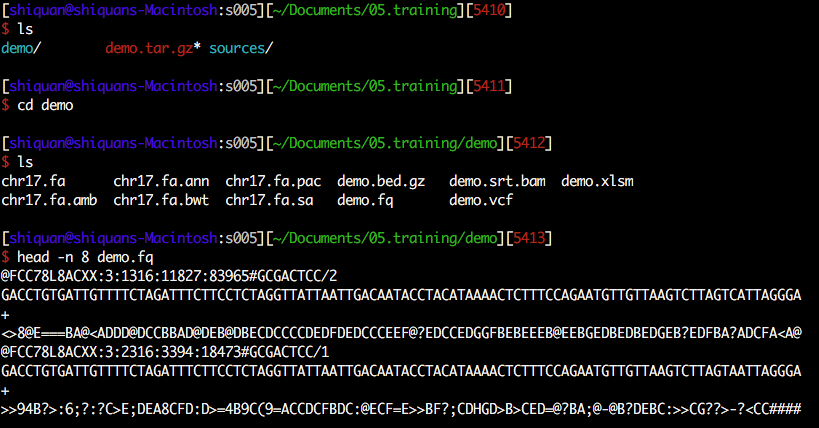
\includegraphics[width=\textwidth]{figures/fastq_com.png}
\end{frame}

\begin{frame}\frametitle{质量值体系}
  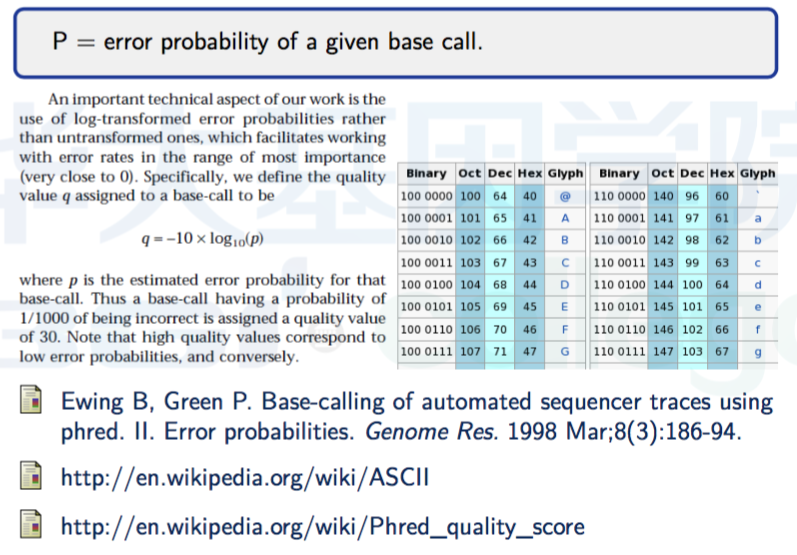
\includegraphics[width=\textwidth]{figures/old_slides/qual1.png}
\end{frame}
\begin{frame}
  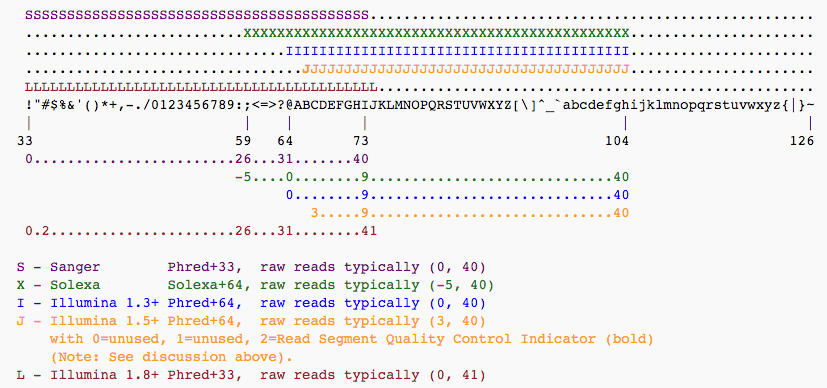
\includegraphics[width=\textwidth]{figures/qual.png}
\end{frame}

\begin{frame}\frametitle{常规重测序分析流程(最简版)}
最终目的就是查找样品与参考序列的不同(变异信息)。
\includegraphics[width=\textwidth]{figures/pipe.pdf}
\end{frame}

\begin{frame}\frametitle{比对}
  {\large{\ttfamily{``The most important first step in understanding next-generation sequencing data is the initial alignment or assembly that determines whether an experiment has succeeded and provides a first glimpse into the results.''\cite{ref2}}}}



  \tikz \node[refbg]{
\begin{thebibliography}{1}
  {\small{\bibitem[Paul F., Ewan B.]{ref2}  Paul Flicek, Ewan Birney. Sense from sequence reads: methods for alignment and assembly. \emph{Nature Methods}, \textbf{Vol 6},  online: 6 May 2010.}}
\end{thebibliography}
};
\end{frame}
\begin{frame}
  \begin{itemize}
  \item  比对即是在参考基因组上查找片段的位置。
  \item 试想,如果是你设计查找软件的话,你会怎么做?
  \end{itemize}

  
  \includegraphics[width=\textwidth]{figures/mapping.pdf}  
  \end{frame}
\begin{frame}\frametitle{比对策略}
  \begin{itemize}
  \item 基于Hash Table的比对算法。
  \item 基于BWT的比对算法。
  \end{itemize}
  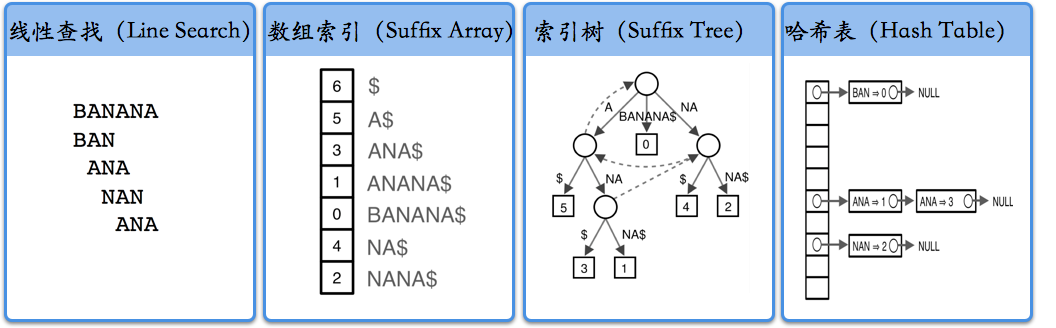
\includegraphics[width=\textwidth]{figures/alignment_algorithms.png}
\end{frame}

\begin{frame}
  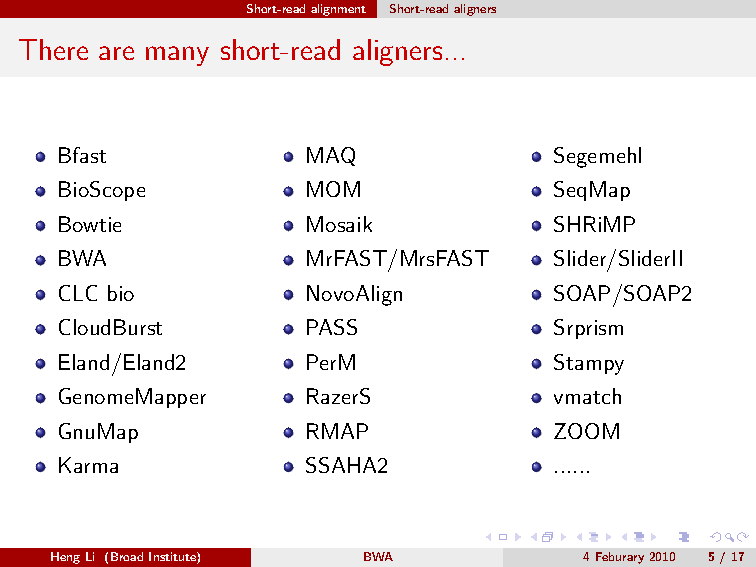
\includegraphics[width=\textwidth]{figures/mapper.pdf}  
  \end{frame}
\begin{frame}\frametitle{参考基因组序列存储格式}
  \begin{itemize}
    \item fasta 格式是目前最通用的参考基因组存储格式。但直接使用数据性能较差。实际使用过程中会根据需要索引或者压缩成各种不同 的格式。
    \item fasta 格式与之前介绍的 fastq 格式类似,但每个条目只有两个数据部分。第一部分是染色体名或者序列名。第二部分为序列信息。
    \item fasta 格式文件在使用中通常先根据需求进行索引。本实验测试比对工具bwa对fasta的索引以及samtools对fasta文件的索引。
\end{itemize}


\end{frame}
\begin{frame}\frametitle{实验上机:查看fasta文件}
  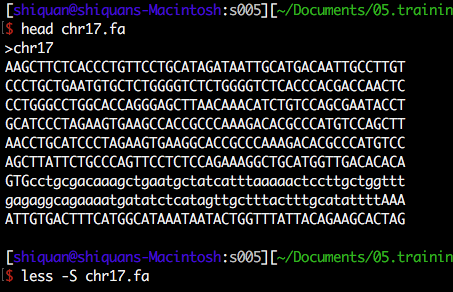
\includegraphics[width=\textwidth]{figures/fasta_com.png}
\end{frame}

\begin{frame}\frametitle{实验上机:参考序列索引}
  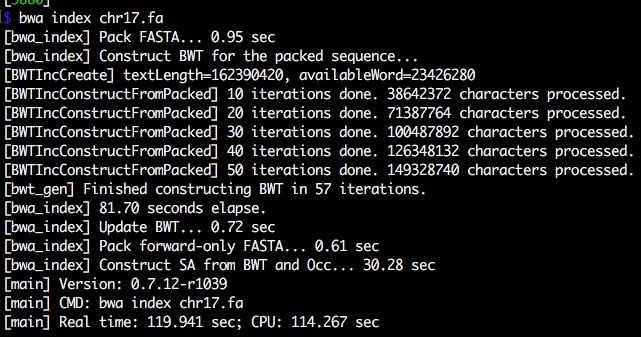
\includegraphics[width=\textwidth]{figures/index_com.png}
\end{frame}

\begin{frame}\frametitle{比对格式}
  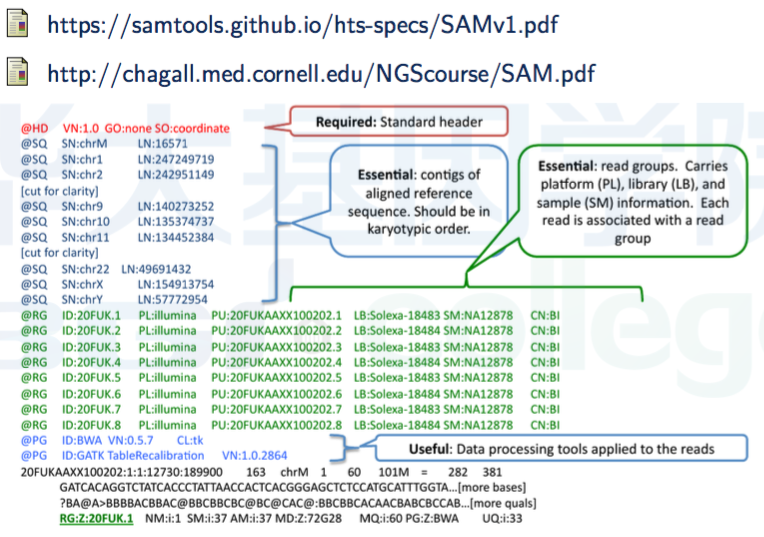
\includegraphics[width=\textwidth]{figures/old_slides/sam.png}
\end{frame}

\begin{frame}
  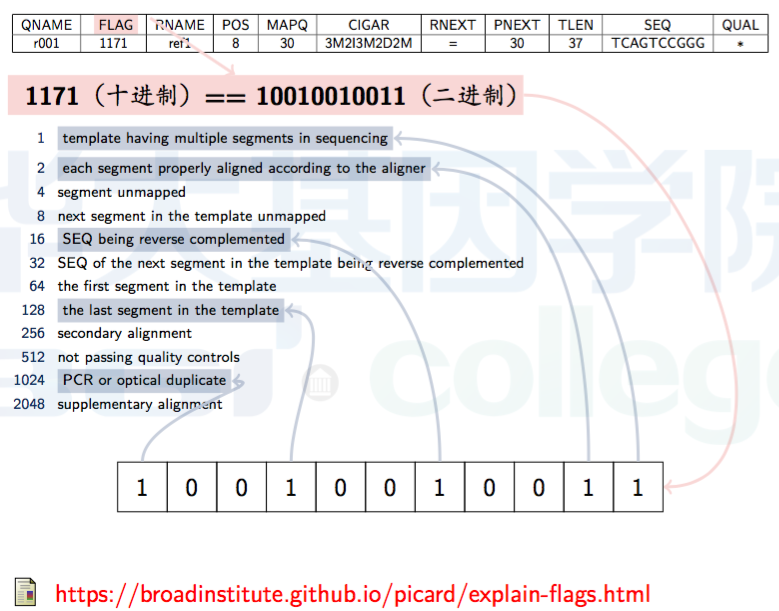
\includegraphics[width=\textwidth]{figures/old_slides/sam-for1.png}
\end{frame}

\begin{frame}
  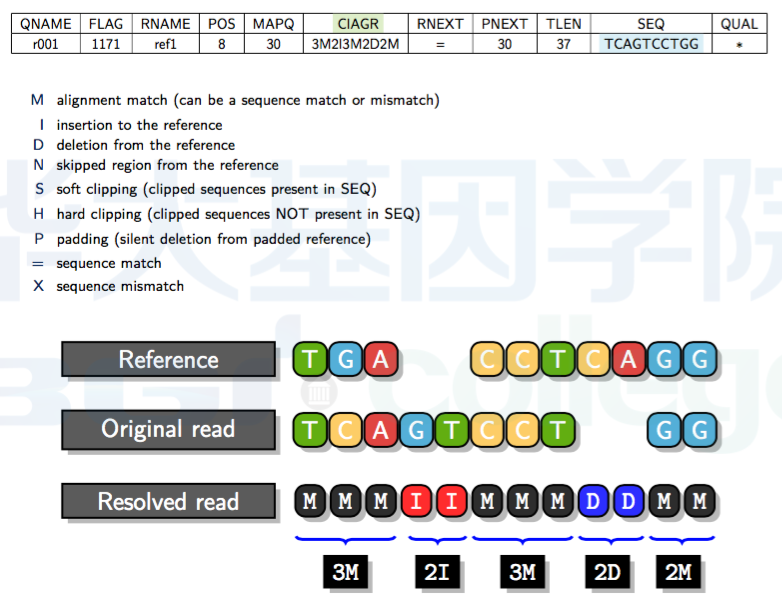
\includegraphics[width=\textwidth]{figures/old_slides/sam-for2.png}
\end{frame}

\begin{frame}
  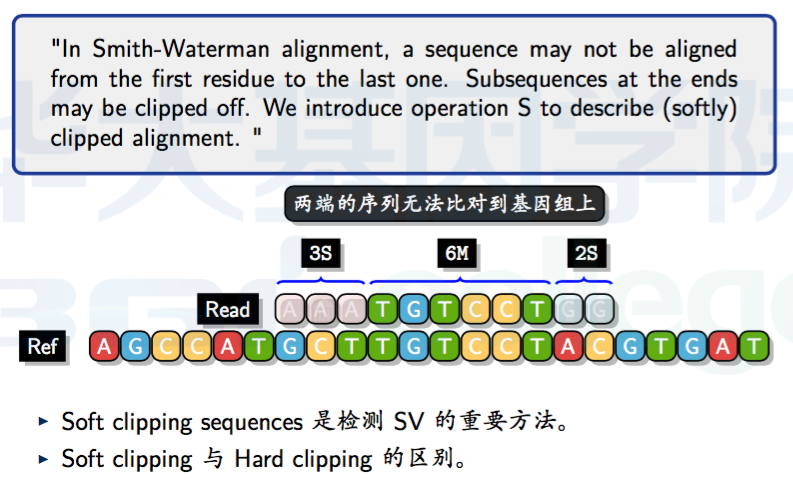
\includegraphics[width=\textwidth]{figures/old_slides/sam-for3.png}
\end{frame}

\defverbatim[colored]\map{
\begin{lstlisting}[language=bash,basicstyle=\ttfamily,keywordstyle=\color{red}]
 $ bwa mem chr17.fa BRCA_demo.fq.gz|samtools view -Sb -|samtools sort - demo.srt
 $ samtools view demo.srt.bam
\end{lstlisting}
}

\begin{frame}\frametitle{实验上机: 比对以及查看SAM/BAM/CRAM文件}
\map

\end{frame}

\begin{frame}\frametitle{比对中常见的问题}
  \begin{itemize}
  \item amplification errors
  \item strand bias
  \item duplicate reads
  \item multireads
  \item chimeric reads
  \item un-properly paired reads    
  \end{itemize}
  \end{frame}

\begin{frame}\frametitle{变异检测}
  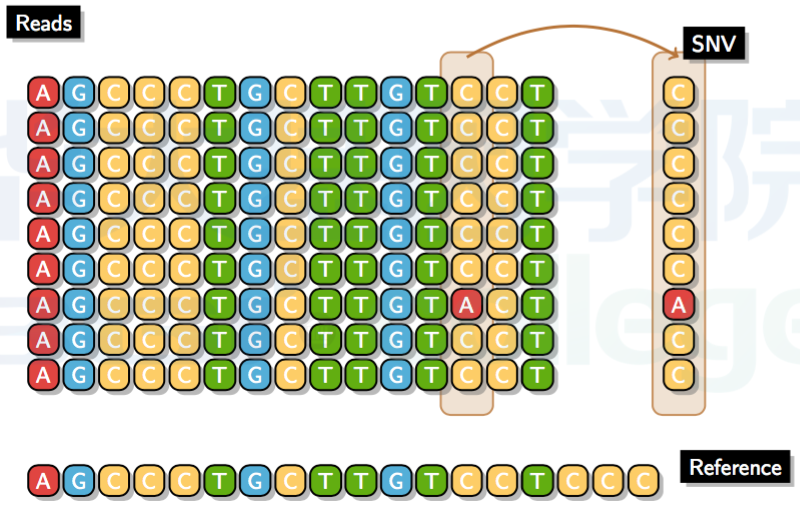
\includegraphics[width=\textwidth]{figures/old_slides/snv1.png}
\end{frame}

\begin{frame}
  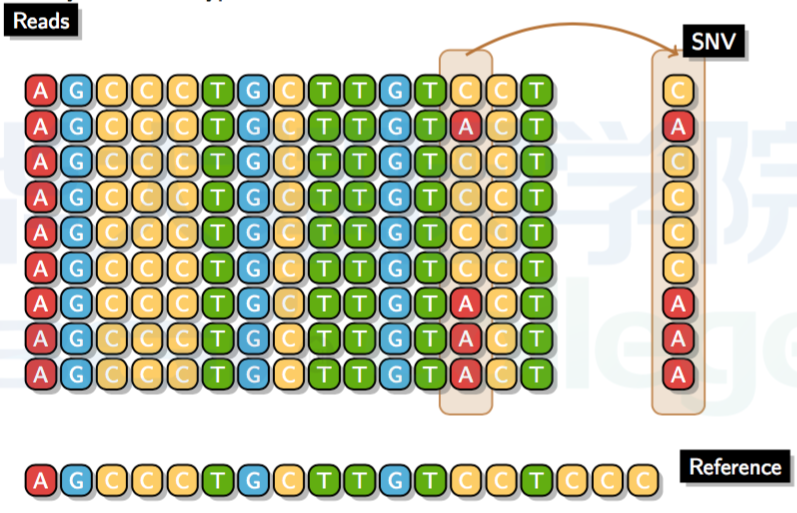
\includegraphics[width=\textwidth]{figures/old_slides/snv2.png}
\end{frame}


\begin{frame}
  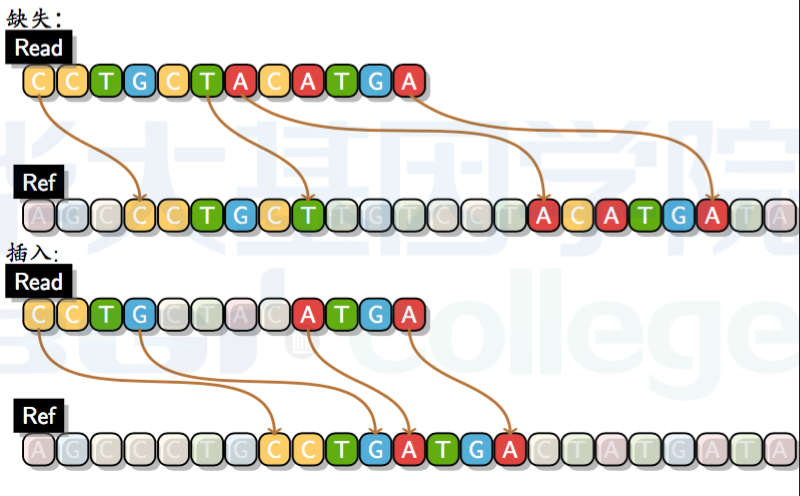
\includegraphics[width=\textwidth]{figures/old_slides/indel1.png}
\end{frame}

\begin{frame}\frametitle{结构变异检测}
  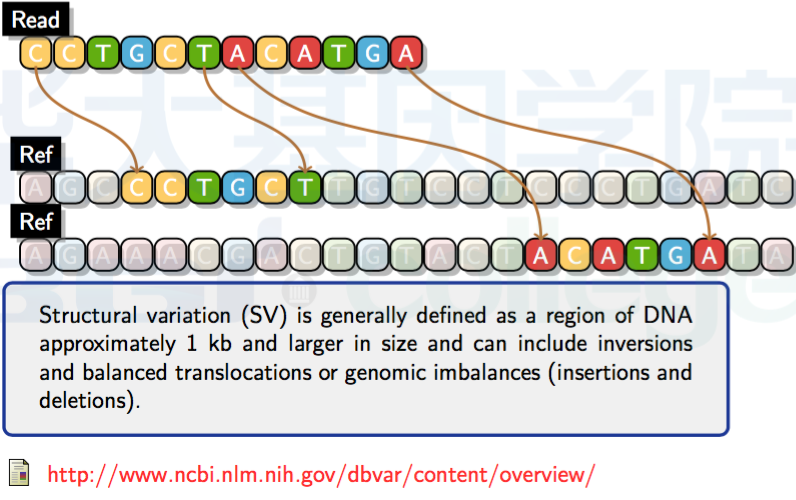
\includegraphics[width=\textwidth]{figures/old_slides/sv.png}  
\end{frame}

\begin{frame}\frametitle{结构变异检测}
  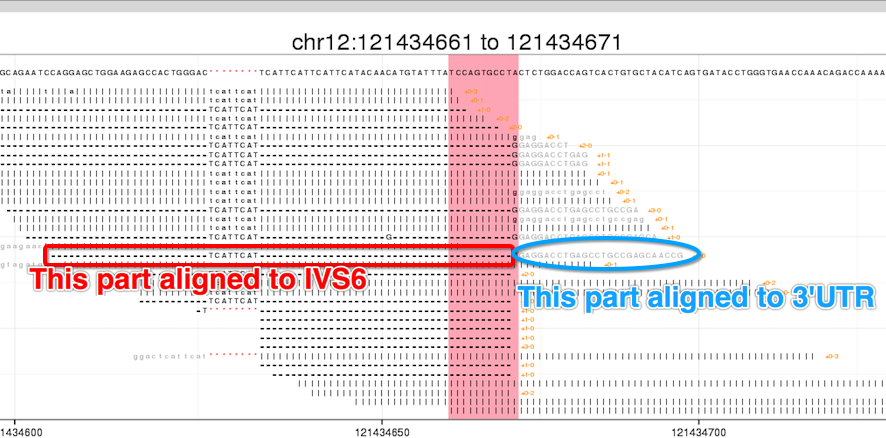
\includegraphics[width=\textwidth]{figures/softclip.png}  
\end{frame}

\begin{frame}\frametitle{染色体拷贝变异检测}
  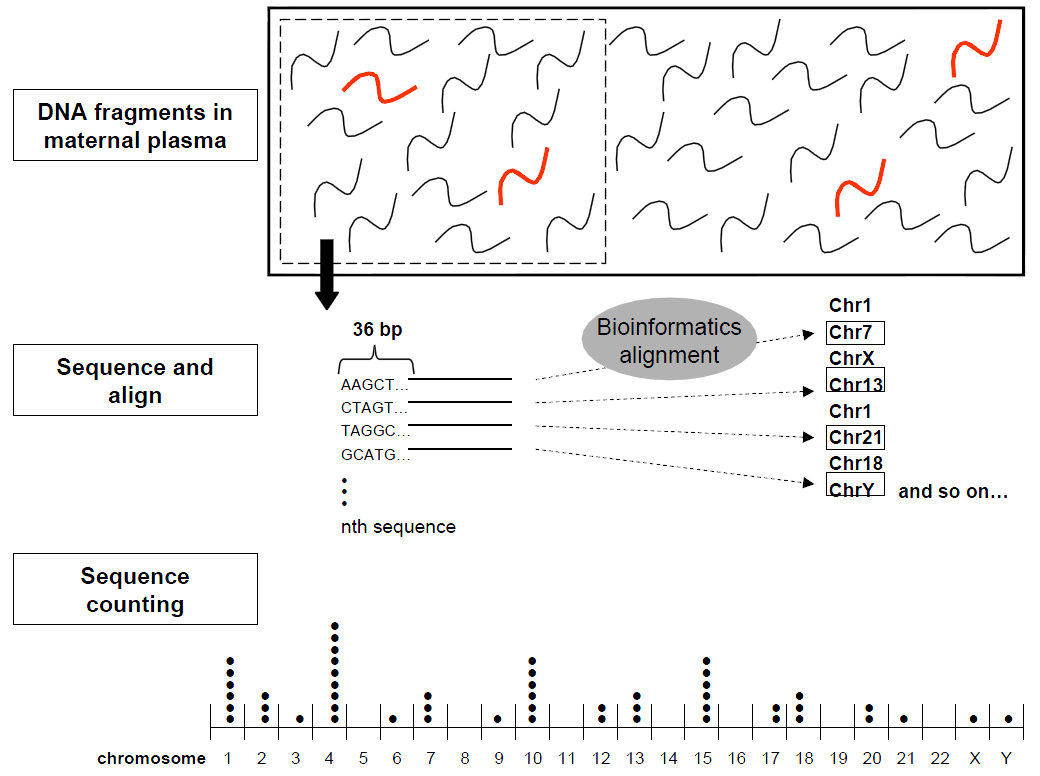
\includegraphics[width=\textwidth]{figures/nift.png}  
\end{frame}


\begin{frame}{CNV检测}
  \begin{itemize}
  \item 利用深度检测;
  \item 利用断裂点检测(同 SV);
  \item 利用突变基因型检测。
  \end{itemize}
  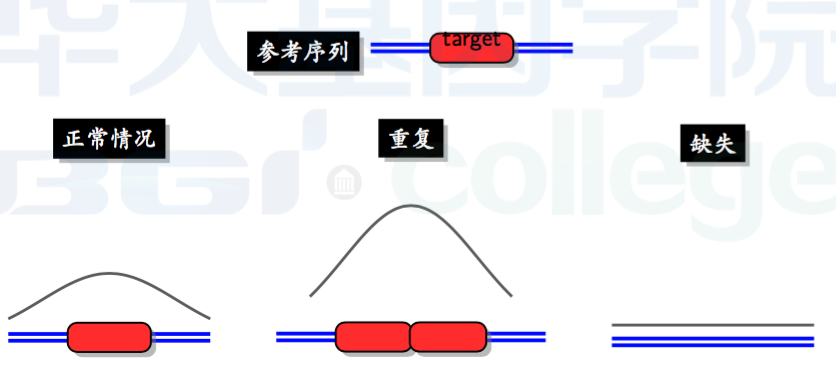
\includegraphics[width=\textwidth]{figures/old_slides/cnv2.png}
\end{frame}

\begin{frame}\frametitle{上机操作:变异检测}
  samtools mpileup -uf chr17.fa.gz demo.srt.bam |bcftools call -cv > demo.vcf
\end{frame}
\begin{frame}\frametitle{变异检测中常见的问题}
  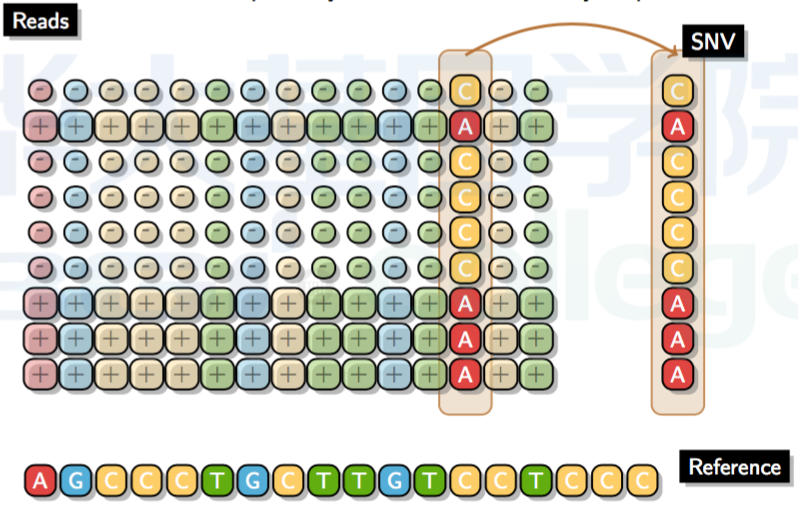
\includegraphics[width=\textwidth]{figures/old_slides/strand.png}
\end{frame}
\begin{frame}\frametitle{变异格式}
  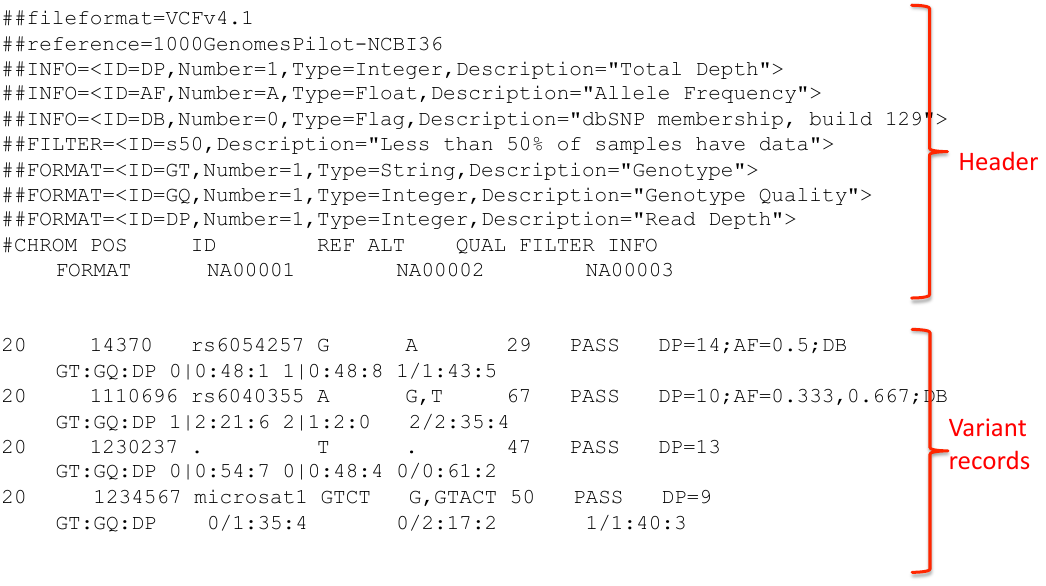
\includegraphics[width=\textwidth]{figures/old_slides/vcf-for.png}
\end{frame}

\begin{frame}\frametitle{重测序分析流程(升级版1.0)}
  \includegraphics[width=\textwidth]{figures/pipe2.pdf}
\end{frame}

\begin{frame}\frametitle{去重复}
  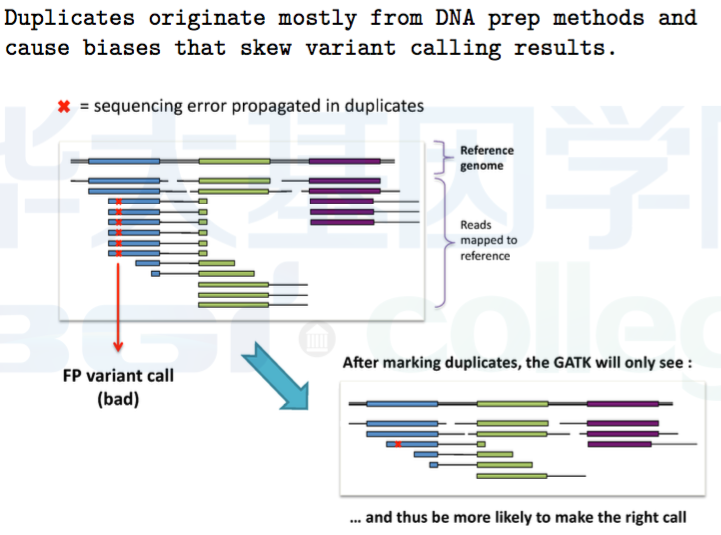
\includegraphics[width=\textwidth]{figures/old_slides/rmdup.png}
\end{frame}

\begin{frame}\frametitle{深度覆盖度统计}
  \begin{itemize}
  \item 目标区域深度计算;
  \item 目标区域内覆盖度;
  \end{itemize}
  \begin{tikzpicture}
    \path[elec] (0,0) node[anchor=south east]{目标区域}  -- ++ (9,0);
    \foreach \i in {1,2,...,6} {
        \path[vib] (2,0 + \i*0.2) -- ++ (6,0);
    }
    \foreach \i in {1,2,...,12} {
        \path[vib] ({4.5 - 1*exp(-0.3*\i)},1.2+\i*0.2) -- (8,1.2+\i*0.2);
    }
    \path[relax] (6,0) -- ++(0,3.6) node[rotate=90,text=orange,pos=0.5,yshift=3mm] {\textbf{测序深度(depth)}};
  \end{tikzpicture}



  https://github.com/shiquan/bamdst
\end{frame}

\begin{frame}\frametitle{重测序分析流程中的质量控制}
  根据使用工具不同,细节有所调整。详细分析步骤请参考GATK以及Picard等工具相关网站资源。
  \begin{itemize}
  \item 测序质量
  \item 深度、覆盖度
  \item 性别预测
  \item 突变信息质控
    \begin{itemize}
    \item Ti/Tv
    \item 突变个数
    \item Read depth
    \item allele balance
    \item strand bias
    \item Genotype quality
    \item HWE
    \item allele frequence (开放数据库中该位点频率)
    \item 其他
    \end{itemize}
    \end{itemize}
\end{frame}

\begin{frame}\frametitle{Burden test}
  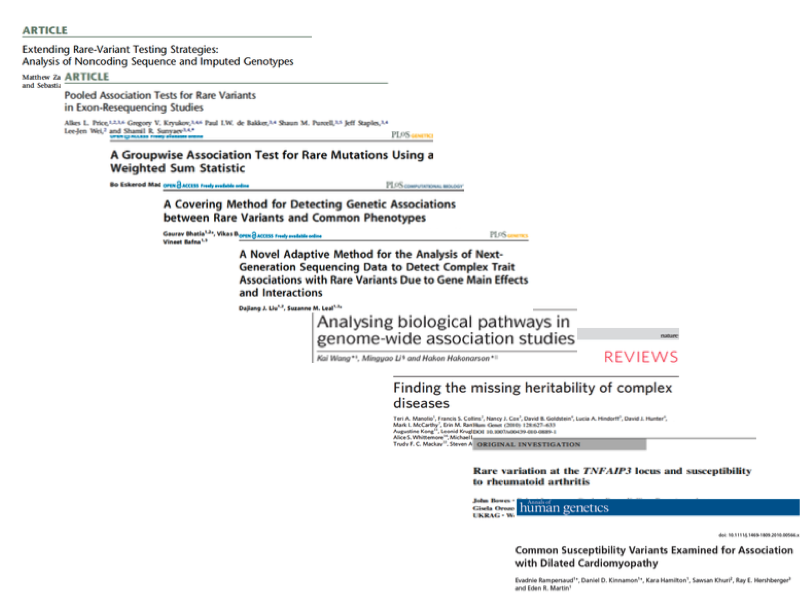
\includegraphics[width=\textwidth]{figures/burdentest.png}
\end{frame}

\begin{frame}\frametitle{重测序分析流程(非人版)}
  \includegraphics[width=\textwidth]{figures/pipe3.pdf}
\end{frame}

\section{为什么重测序的工作中也需要组装技术?}
\begin{frame}\frametitle{为什么重测序的工作中也需要组装技术?}
由于目前测序读长仍然较短,对于大范围的变异检测受限。将多条短序列连接成长序列,再和基因组进行比较,从而达到检测大范围结构变异的目的。常用软件如Pindel。
\end{frame}

\section{测序分析流程回顾}

\begin{frame}\frametitle{测序分析流程回顾}
  \begin{columns}
    \begin{column}{0.5\textwidth}
      \includegraphics[width=\textwidth]{figures/pip_layer.pdf}      
    \end{column}
    \begin{column}{0.5\textwidth}
      \begin{enumerate}
      \item 下机过滤
      \item 比对
      \item 深度覆盖度计算
      \item 变异检测
      \item 注释
      \end{enumerate}
    \end{column}
  \end{columns}
\end{frame}

\section{变异注释}
\begin{frame}\frametitle{变异注释}
  \begin{columns}
    \begin{column}{0.35\textwidth}
\begin{itemize}
  \item 功能丧失突变
  \item 功能获得突变
  \item 显性失活突变
  \item 单倍剂量不足
\end{itemize}
    \end{column}
    \begin{column}{0.7\textwidth}
      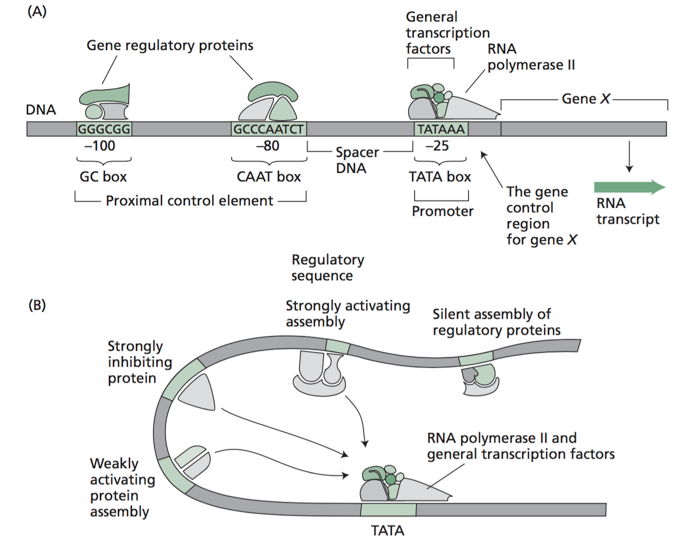
\includegraphics[width=\textwidth]{figures/func.png}  
    \end{column}
  \end{columns}
  PLANT PSYSIOLOGY, 3rd edition, Figure 14.6
\end{frame}
\begin{frame}\frametitle{HGVS命名}
    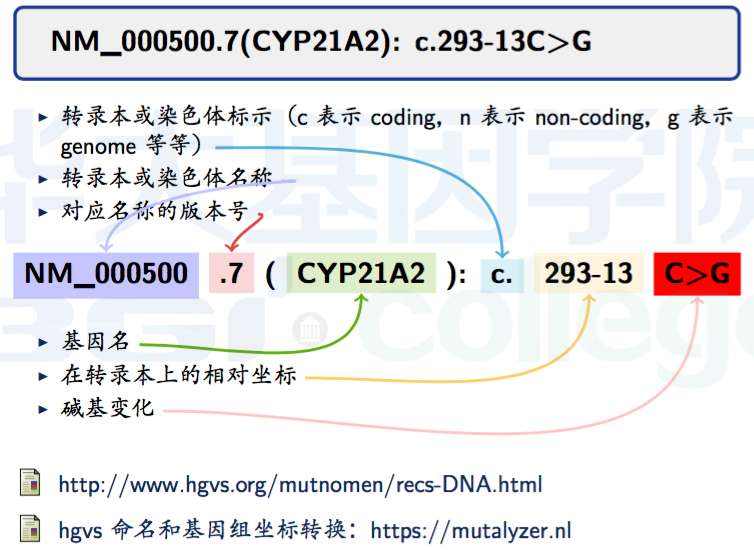
\includegraphics[width=\textwidth]{figures/old_slides/hgvs.png}  
  \end{frame}
\begin{frame}\frametitle{变异注释}
  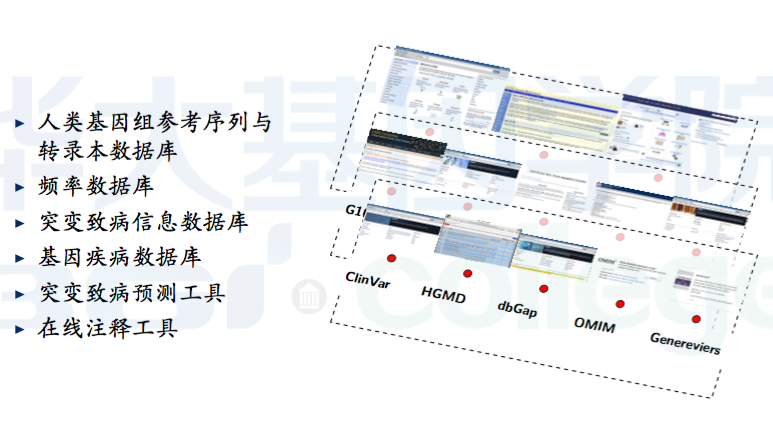
\includegraphics[width=\textwidth]{figures/old_slides/anno1.png}  
\end{frame}

\begin{frame}
  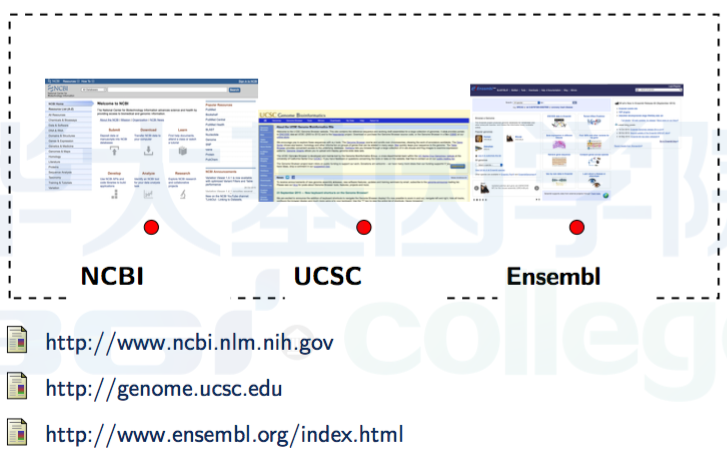
\includegraphics[width=\textwidth]{figures/old_slides/anno2.png}  
\end{frame}

\begin{frame}
  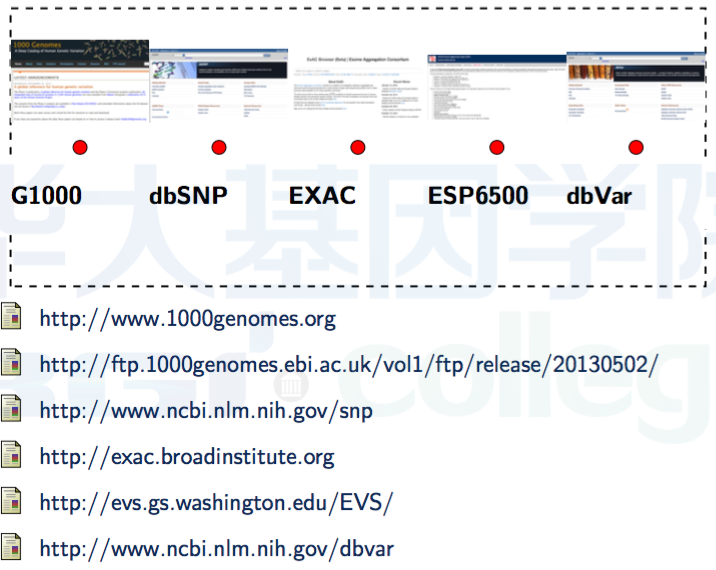
\includegraphics[width=\textwidth]{figures/old_slides/anno3.png}  
\end{frame}

\begin{frame}
  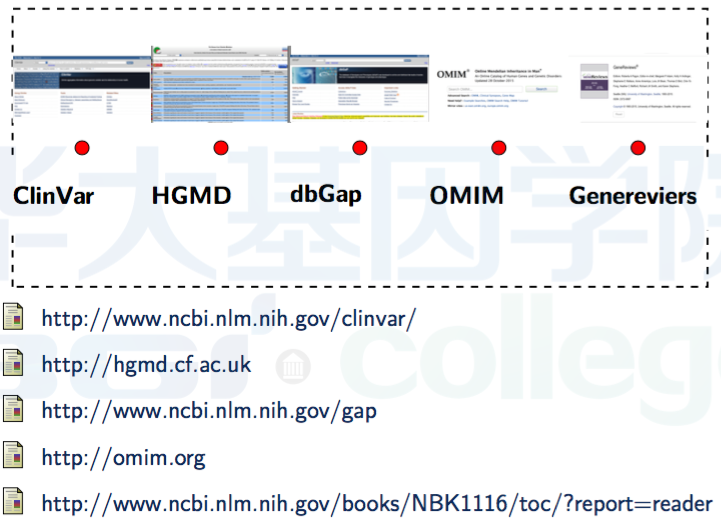
\includegraphics[width=\textwidth]{figures/old_slides/anno4.png}  
\end{frame}

\begin{frame}\frametitle{上机:注释}
  \small{
  \begin{itemize}
    \item http://www.ncbi.nlm.nih.gov/variation/view/
    \item http://www.ensembl.org/info/docs/tools/vep/index.html
    \item http://snp.gs.washington.edu/SeattleSeqAnnotation138/index.jsp
  \end{itemize}
  }
\end{frame}
\begin{frame}\frametitle{ENCODE}
  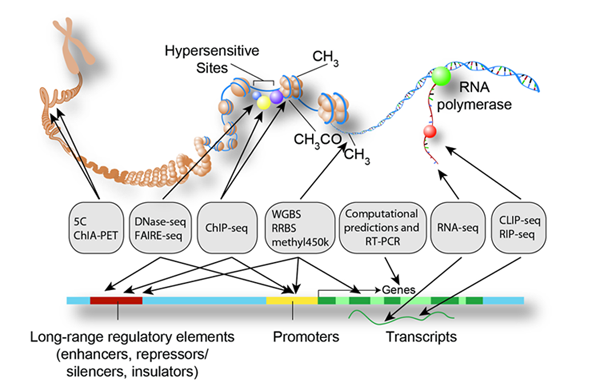
\includegraphics[width=\textwidth]{figures/encode.png}  
\end{frame}
\section{案例分享}
\begin{frame}\frametitle{案例分享}
  \begin{itemize}
  \item DMD检测项目;
  \item 耳聋筛查项目;
  \item 新生儿筛查项目;
  \item MODY检测项目;
  \item 其他项目。
  \end{itemize}
\end{frame}
\section{DNA重测序分析面临的各自挑战}
\begin{frame}\frametitle{Mapping VS. Alignment}
  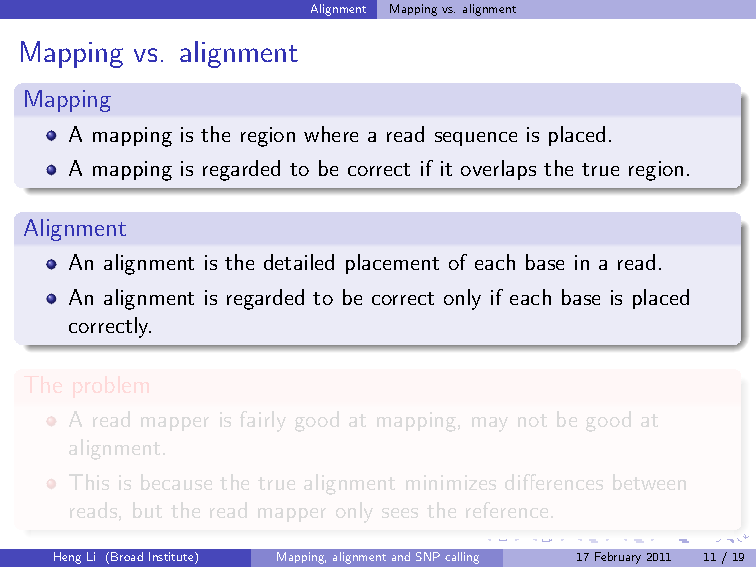
\includegraphics[width=\textwidth]{figures/mappingalign.pdf}  
\end{frame}
\begin{frame}\frametitle{人类基因组参考序列}
  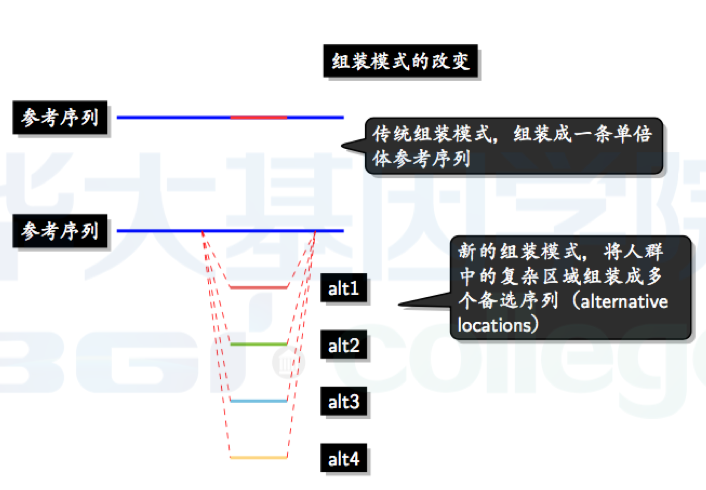
\includegraphics[width=\textwidth]{figures/old_slides/humanref.png}  
\end{frame}

\begin{frame}\frametitle{还有。。}
  \begin{enumerate}
  \item 全基因组测序数据量大,分析占用资源高。怎么破?
    \begin{itemize}
      \item 了解多进程。
      \item 了解Hadoop架构。
      \item 了解云计算(BGI online)。
    \end{itemize}
  \item 目标区域捕获测序面临的最主要的问题是如果保证区域的准确以及捕获的有效数据量高。
    \begin{itemize}
    \item 目标区域定位与提取。
    \item 探针/引物设计。
    \end{itemize}
  \end{enumerate}
\end{frame}

\section{研究思路与整体流程回顾}
\begin{frame}\frametitle{研究思路与整体流程回顾}
  \begin{itemize}
  \item 研究目的是什么?
  \item 对象和样品是?
  \item 参考序列有么?
  \item 数据量多少?
  \item WGS? WES? PCR?
  \item 筛查还是诊断?
  \end{itemize}
\end{frame}

\begin{frame}\frametitle{建库方法,插入片段与分析策略}
  \begin{itemize}
  \item 测什么?对读长有要求么?
  \item 有什么测序平台可选?
  \item 建库时间考虑么?
  \end{itemize}
  
\end{frame}

\begin{frame}\frametitle{比对策略与适用范围}
  \begin{itemize}
  \item 测序读长多少?
  \item 测序质量如何?
  \item 物种变异几率如何?参考序列准确性如何?
  \item 灵敏度和速度怎么分配?
    \end{itemize}
\end{frame}

\begin{frame}\frametitle{变异类型与检测方案}
\begin{itemize}
\item SNP检测有哪些要注意的地方?
\item Indel检测呢?
\item CNV?
\item 结构变异?
\end{itemize}
\end{frame}

\begin{frame}\frametitle{注释数据库与解读}
  \begin{itemize}
\item 什么检测项目?单病还是癌症?
\item 要检查somatic还是driver mutations?
\item 产前?孕期?新生儿?
\item 筛查还是诊断?  
\end{itemize}

\end{frame}

\begin{frame}
  \begin{columns}
    \begin{column}{0.5\textwidth}
      \huge{Question \& Discussion}

      
    \end{column}
    \begin{column}{0.5\textwidth}
        
\includegraphics[width=\textwidth]{figures/wchat.jpg}  
    \end{column}

  \end{columns}
  \end{frame}
\end{document}
